\documentclass[a4paper,10pt]{article}
\usepackage{luatexja}
\usepackage{luatexja-fontspec}
\usepackage{geometry}
\usepackage{multicol}
\usepackage{titlesec}
\usepackage{setspace}
\usepackage{graphicx}
\usepackage{caption}
\usepackage{indentfirst}
\usepackage{float} % 図の位置を制御するために追加
\usepackage{listings}
\usepackage{xcolor}
\usepackage{amsmath} % align 環境などの数式用
\usepackage{hyperref}

\geometry{margin=20mm}
\setstretch{1.2}
\parindent=1em

% ===== 日本語フォント設定 =====
% HaranoAjiMincho がシステムに入っている必要あり
\setmainjfont{HaranoAjiMincho} % メイン日本語フォント
\setsansjfont{HaranoAjiGothic} % サンセリフ（任意）
\setmonojfont{HaranoAjiMincho} % 等幅も同じに設定（好みに応じて変更）

% 図のキャプションの表記を「図1」のように日本語化
\renewcommand{\figurename}{図}
\captionsetup[figure]{labelformat=default,labelsep=period}

\renewcommand{\tablename}{表}
\captionsetup[table]{labelformat=default,labelsep=period}

\geometry{margin=25mm}
\setstretch{1.2}
\parindent=1em

\titleformat{\section}{\large\bfseries}{\thesection.}{1em}{}

\definecolor{keywordcolor}{rgb}{0.26, 0.38, 0.68}
\definecolor{commentcolor}{rgb}{0.3, 0.6, 0.3}
\definecolor{stringcolor}{rgb}{0.7, 0.2, 0.2}

\lstdefinelanguage{SystemVerilog}{
  morekeywords={module,endmodule,input,output,logic,always_ff,if,else,begin,end,posedge,negedge},
  sensitive=true,
  morecomment=[l]{//},
  morecomment=[s]{/*}{*/},
  morestring=[b]",
}

\lstset{
  language=SystemVerilog,
  basicstyle=\ttfamily\small,
  keywordstyle=\color{keywordcolor}\bfseries,
  commentstyle=\color{commentcolor}\itshape,
  stringstyle=\color{stringcolor},
  numbers=left,
  numberstyle=\tiny,
  stepnumber=1,
  numbersep=5pt,
  frame=single,
  tabsize=2,
  showstringspaces=false,
  breaklines=true,
  breakatwhitespace=true
}

% -------------------------------------------
% Python 用の listings 言語定義
% -------------------------------------------
\lstdefinelanguage{PythonCustom}{
  language=Python,
  morekeywords={
    def,class,return,import,from,as,with,for,while,if,elif,else,
    try,except,finally,raise,pass,break,continue,lambda,yield,global,nonlocal
  },
  sensitive=true,
  morecomment=[l]{\#},
  morestring=[b]",
}

% -------------------------------------------
% Python 用スタイル
% （SystemVerilog のスタイルを完全踏襲）
% -------------------------------------------
\lstdefinestyle{pythonstyle}{
  language=PythonCustom,
  basicstyle=\ttfamily\small,
  keywordstyle=\color{keywordcolor}\bfseries,
  commentstyle=\color{commentcolor}\itshape,
  stringstyle=\color{stringcolor},
  numbers=left,
  numberstyle=\tiny,
  stepnumber=1,
  numbersep=5pt,
  frame=single,
  tabsize=2,
  showstringspaces=false,
  breaklines=true,
  breakatwhitespace=true
}

\title{パワーエレクトロニクスI 課題2 レポート}
\author{学生番号： 4321 \quad 氏名： 野秋林太郎}
\date{令和7年11月28日}

\begin{document}

\maketitle

\section{等価回路と状態方程式}
スイッチがONのときと、OFFのときの等価回路を図\ref{fig:equivalent_circuits}に示す。

\begin{figure}[htbp]
  \centering
  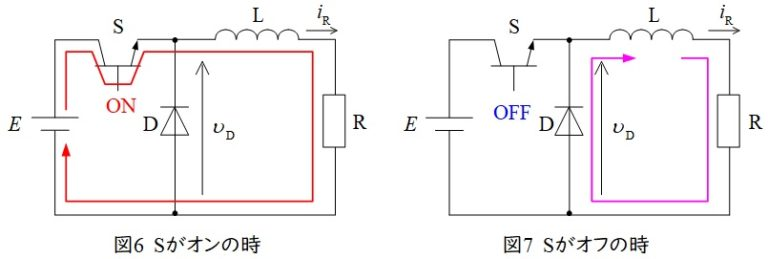
\includegraphics[width=12cm]{aaa.jpg}
  \caption{スイッチON/OFF時の等価回路}
  \label{fig:equivalent_circuits}
\end{figure}

\subsection{スイッチ $S$ がONのとき ($0 \le t < T_{on}$)}
スイッチ $S$ が導通し、電源 $E$ からリアクトル $L$、負荷 $R$ へ電流が流れる。ダイオード $D$ には逆電圧 $E$ が印加されるため遮断状態となる。
キルヒホッフの電圧則より、以下の電圧方程式が成り立つ。

\begin{equation}
    E = L \frac{di_L}{dt} + R i_L
    \label{eq:on_state}
\end{equation}

これがON期間における状態方程式である。

\subsection{スイッチ $S$ がOFFのとき ($T_{on} \le t < T$)}
スイッチ $S$ が遮断されると、リアクトル $L$ の電流連続性により、ダイオード $D$ が導通（還流）する。電源 $E$ は切り離されるため、回路への入力電圧は0となる（ダイオードの順方向電圧降下を無視する）。
このときの電圧方程式は以下の通りである。

\begin{equation}
    0 = L \frac{di_L}{dt} + R i_L
    \label{eq:off_state}
\end{equation}

これがOFF期間における状態方程式である。

\section{定常状態における負荷電流 $i_L(t)$ の導出}
定常状態における電流波形を求める。時定数を $\tau = L/R$ と置く。

\subsection{ON期間 ($0 \le t \le T_{on}$)}
式(\ref{eq:on_state})は一階線形微分方程式である。一般解は定数 $K_1$ を用いて次式で表される。
\begin{equation}
    i_L(t) = \frac{E}{R} + K_1 e^{-\frac{t}{\tau}}
\end{equation}
初期条件 $i_L(0) = I_{min}$ より、$K_1$ を求める。
\begin{equation}
    I_{min} = \frac{E}{R} + K_1 \quad \therefore K_1 = I_{min} - \frac{E}{R}
\end{equation}
よって、ON期間の電流 $i_L(t)$ は次式となる。
\begin{equation}
    i_L(t) = \frac{E}{R} + \left( I_{min} - \frac{E}{R} \right) e^{-\frac{t}{\tau}} \quad (0 \le t \le T_{on})
    \label{eq:il_on}
\end{equation}

\subsection{OFF期間 ($T_{on} \le t \le T$)}
式(\ref{eq:off_state})の一般解は定数 $K_2$ を用いて次式で表される。
\begin{equation}
    i_L(t) = K_2 e^{-\frac{t}{\tau}}
\end{equation}
ここで、ON期間終了時の電流値 $i_L(T_{on}) = I_{max}$ を境界条件として用いる。
\begin{equation}
    I_{max} = K_2 e^{-\frac{T_{on}}{\tau}} \quad \therefore K_2 = I_{max} e^{\frac{T_{on}}{\tau}}
\end{equation}
よって、OFF期間の電流 $i_L(t)$ は次式となる。
\begin{equation}
    i_L(t) = I_{max} e^{-\frac{t - T_{on}}{\tau}} \quad (T_{on} \le t \le T)
    \label{eq:il_off}
\end{equation}

\section{$I_{max}$ と $I_{min}$ の導出}
回路定数を用いて $I_{max}$ と $I_{min}$ を決定する。

式(\ref{eq:il_on})において $t=T_{on}$ のとき $i_L(T_{on}) = I_{max}$ となることから、
\begin{equation}
    I_{max} = \frac{E}{R} + \left( I_{min} - \frac{E}{R} \right) e^{-\frac{T_{on}}{\tau}}
    \label{eq:imax_temp}
\end{equation}
また、式(\ref{eq:il_off})において $t=T$ のとき $i_L(T) = I_{min}$ となることから（定常状態の周期性）、
\begin{equation}
    I_{min} = I_{max} e^{-\frac{T - T_{on}}{\tau}} = I_{max} e^{-\frac{T_{off}}{\tau}}
    \label{eq:imin_temp}
\end{equation}
式(\ref{eq:imin_temp})を式(\ref{eq:imax_temp})に代入して整理する。
\begin{align}
    I_{max} &= \frac{E}{R} (1 - e^{-\frac{T_{on}}{\tau}}) + I_{max} e^{-\frac{T_{off}}{\tau}} e^{-\frac{T_{on}}{\tau}} \\
    I_{max} (1 - e^{-\frac{T}{\tau}}) &= \frac{E}{R} (1 - e^{-\frac{T_{on}}{\tau}})
\end{align}
これより $I_{max}$ が求まる。
\begin{equation}
    I_{max} = \frac{E}{R} \frac{1 - e^{-\frac{R}{L} T_{on}}}{1 - e^{-\frac{R}{L} T}}
\end{equation}
同様に $I_{min}$ は次式となる。
\begin{equation}
    I_{min} = \frac{E}{R} \frac{e^{\frac{R}{L} T_{on}} - 1}{e^{\frac{R}{L} T} - 1}
\end{equation}

\section{数値シミュレーションと波形\footnote{このセクションはExcelではなく、Pythonでシミュレーションを行いました。}}
以下の回路定数を設定し、電圧・電流波形を作成した。

\begin{itemize}
    \item 入力電圧 $E = 100$ [V]
    \item 負荷抵抗 $R = 10$ [$\Omega$]
    \item リアクトル $L = 1$ [mH]
    \item スイッチング周波数 $f = 10$ [kHz] (周期 $T = 100$ [$\mu$s])
    \item 時比率 $d = 0.5$ ($T_{on} = 50$ [$\mu$s])
\end{itemize}

図\ref{fig:waveforms}に定常状態における出力電圧および負荷電流の波形を示す。
電流は連続モードで動作しており、計算された $I_{max}, I_{min}$ の間で指数関数的に脈動していることが確認できる。

\begin{figure}[htbp]
  \centering
  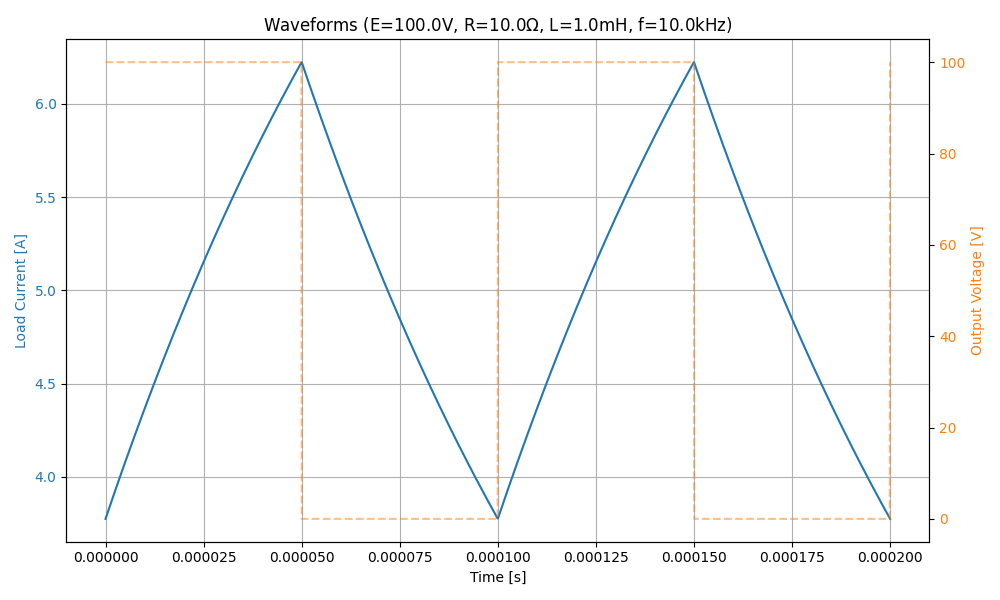
\includegraphics[width=12cm]{waveform.png}
  \caption{出力電圧と負荷電流の波形 (d=0.5)}
  \label{fig:waveforms}
\end{figure}

\section{デューティー比と出力電圧平均値\footnote{このセクションはExcelではなく、Pythonでシミュレーションを行いました。}}
デューティー比 $d$ を $0$ から $1.0$ まで $0.1$ 刻みで変化させたときの出力電圧平均値 $V_{avg}$ の関係を図\ref{fig:avg_voltage}に示す。
理論式 $V_{avg} = d E$ に従い、デューティー比に対して出力電圧が線形に変化していることがわかる。
\begin{figure}[htbp]
  \centering
  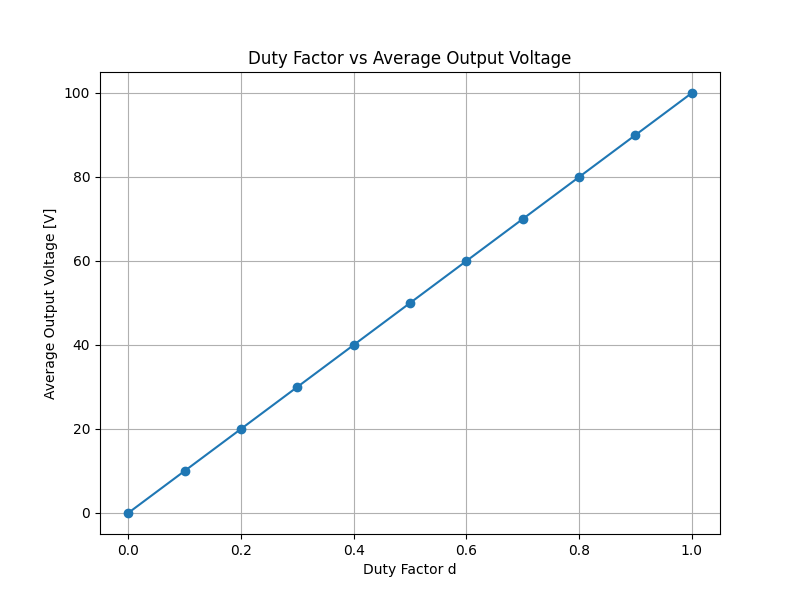
\includegraphics[width=10cm]{avg_voltage.png}
  \caption{デューティー比と出力電圧平均値の関係}
  \label{fig:avg_voltage}
\end{figure}

\section{リプルの低減手法\footnote{このセクションはExcelではなく、Pythonでシミュレーションを行いました。}}
出力電流のリプルを小さくするための手法として、主に以下の2点が挙げられる。

\begin{enumerate}
    \item \textbf{リアクトル $L$ のインダクタンスの増加}: 時定数 $\tau = L/R$ を大きくすることで、電流変化の傾きを緩やかにし、リプル幅を低減する。
    \item \textbf{スイッチング周波数の高周波化}: 周期 $T$ を短くすることで、電流が増加・減少する時間を短縮し、振幅が大きくなる前にスイッチングを行うことでリプル幅を低減する。
\end{enumerate}

それぞれの効果を検証するため、初期設定 ($L=1$ mH, $f=10$ kHz) を基準とし、パラメータを変更した場合の比較を行った。

\subsection{インダクタンスによる効果}
図\ref{fig:ripple_L}に、インダクタンスを10倍の $L=10$ [mH] に変更した場合の比較結果を示す。
$L$ を大きくすることで電流の傾きが緩やかになり、リプル成分が著しく減少していることが確認できる。

\begin{figure}[htbp]
  \centering
  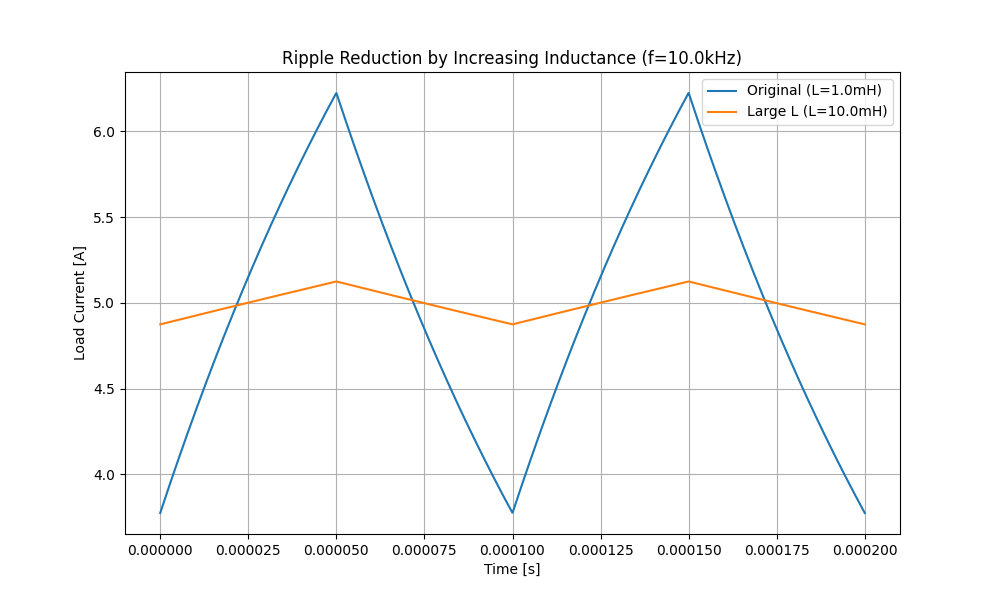
\includegraphics[width=12cm]{ripple_comparison_L.png}
  \caption{インダクタンス変更による電流リプルの比較 ($L=1$mH vs $10$mH)}
  \label{fig:ripple_L}
\end{figure}

\subsection{スイッチング周波数による効果}
図\ref{fig:ripple_F}に、スイッチング周波数を10倍の $f=100$ [kHz] に変更した場合の比較結果を示す。
周波数を高くすることで充放電のサイクルが短くなり、結果として電流の脈動幅が大幅に圧縮されていることがわかる。
なお、周波数を上げても平均電流値には変化がないことも確認できる。

\begin{figure}[htbp]
  \centering
  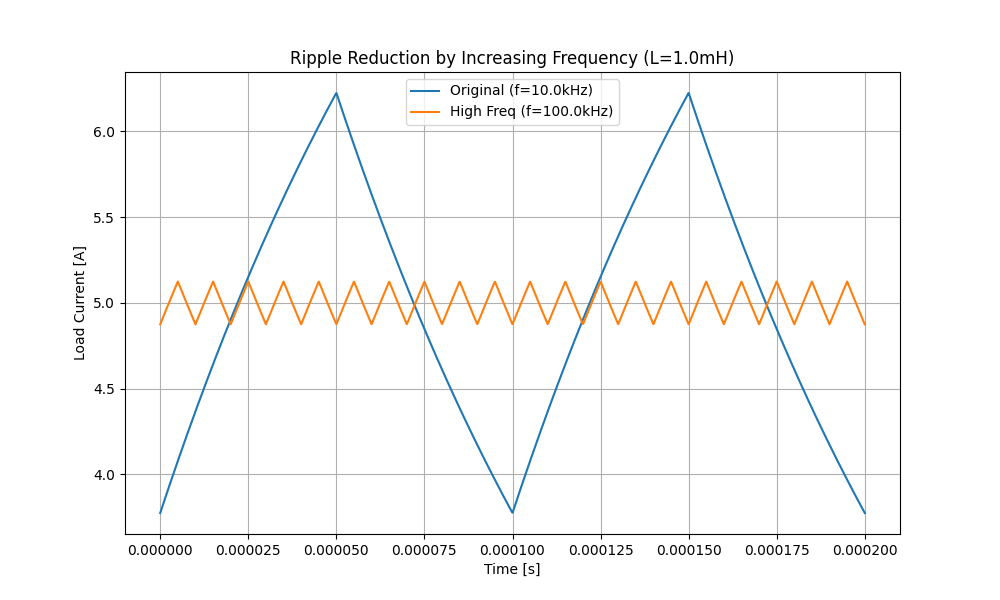
\includegraphics[width=12cm]{ripple_comparison_F.png}
  \caption{スイッチング周波数変更による電流リプルの比較 ($f=10$kHz vs $100$kHz)}
  \label{fig:ripple_F}
\end{figure}

\end{document}